\chapter{Imitation Dynamics}
	\section{Θεωρητική ανάλυση του Imitation Dynamics:}
	
	Σε αυτό το σημείο θα αναλύσουμε τη θεωρητική ανάλυση του Imitation Dynamics.  Aυτό περιλαμβάνει την δημιουργία ενός πίνακα μεταβάσεων μιας αλυσίδας Markov. Παρακάτω θα αναλύσουμε πως λειτουργεί αυτή η μέθοδος παραγωγής του πίνακα μεταβάσεων.
	\\
	
	Παρακάτω ο κώδικας της συνάρτησης \nameref{appendix:TTI}:
	\\

	
	
	\indent Παμε να δουμε αναλυτικά γραμμή προς γραμμή:
	
	Αρχικα καλούμε την συνάρτηση \nameref{appendix:ACS}, η οποία δίνει όλες τις πιθανές καταστάσεις της διαδικασίας Markov, της οποίας τον πίνακα μεταβάσεων αναζητούμε .
	\\
	
	

	


	\vspace{1em}
	
	Η συνάρτηση ακολουθεί την λογική του \textit{stars and bars problem} για να υπολογίσει ολους τους πιθανούς συνδυασμούς θετικών αριθμων που αθροίζουν στον πληθυσμο που έχουμε βάλει σαν όρισμα.
	\\
	\\
	Προχωρώντας στις επόμενες γραμμές: Αρχικοποιούμε τον πίνακα μεταβάσεων και ξεκινάμε μια \texttt{for} loop για κάθε γραμμή του πίνακα, (δηλαδή για κάθε συνδυασμό των combos).
	\\
	\\
Εντός της λούπας: Υπολογίζουμε τα scores για κάθε στρατηγική με την συνάρτηση \nameref{appendix:A2I}.
\\
\\
	Η βελτιωμένη αυτή εκδοση αξιοποιεί την ανάλυση από το \texttt{TourTheFit} για να υπολογίσει με μεγαλύτερη ταχύτητα τα Scores για κάθε στρατηγική.

	Επειτα , με την συνάρτηση \nameref{appendix:FBIS} βρίσκω τις στρατηγικές (μια η περισσότερες) που είναι βέλτιστες. Επιπλέον υπολογίζει και τις υποβελτιστες στρατηγικές(θα μας χρησιμεύσουν μετα).\\
	

	Προχωρώντας, χρησιμοποιώντας την \nameref{appendix:ASstr} , την οποία έχουμε υλοποιήσει για το πρωτάθλημα Axelrod της 1ης εργασίας, μετατρέπουμε την μορφή:
	
	\[X(t_i)=\Bigl(x_1(t_i),x_2(t_i),\dotsc,x_m(t_i)\Bigr)\to Y(t_i)=\underbrace{\texttt{str}_1,\dots\texttt{str}_1}_{x_1(t_i) \text{ times }}\ , \ \underbrace{\texttt{str}_2,\dots\texttt{str}_2}_{x_2(t_i) \text{ times }}\ , \dots,\underbrace{\texttt{str}_m,\dots\texttt{str}_m}_{x_m(t_i) \text{ times }} \]
	\\
	Η μορφή αυτή εξυπηρετεί τους εξής σκοπούς:
	\begin{itemize}
		\item Είναι ευκολότερη η εύρεση πιθανών μεταβολών παιχτών
		\\
		\item Δεν μας ενδιαφέρει η διάταξη των στοιχείων. Όπως είχαμε αναφέρει στο μάθημα, η διαδικασία markov για τις καταστάσεις \(Y\) (ας τις ονομάσουμε \texttt{r\_states} έναντι των \texttt{s\_states}) είναι lumpable σε σχέση με τα
		\texttt{s\_states} \footnote{βλέπε στο Appendix για λεπτομέρειες} Αυτό σημαίνει ότι το άθροισμα των πιθανοτήτων μεταβολών ενος συγκεκριμένου \texttt{group r\_states} που αναπαριστούν ένα συγκεκριμένο \texttt{s\_state} είναι σταθερό από  οποιαδήποτε άλλη κατάσταση ενος συγκεκριμένου \texttt{s\_state} και να προερχόμαστε.
		
		
	\end{itemize}

	Παρακάτω, εφόσον έχουμε τώρα το \texttt{r\_state}, υπολογίζουμε τα \textit{indexes} που αντιστοιχούν σε βέλτιστες και υποβέλτιστες στρατηγικές. Εδώ κάνουμε και μια παραδοχή για να μπορέσει ο μηχανισμός μας να αντιμετωπίσει ειδικες περιπτώσεις: Εφόσον ο αριθμός υποβέλτιστων παιχτών είναι μικρότερος από \(Κ\), τότε σαν υποψήφιοι παίκτες προς αλλαγή στρατηγικής συμπεριλαμβάνονται και οι βελτιστοι παίκτες(δηλαδή όλοι οι παίκτες είναι υποψήφιοι για αλλαγή στρατηγικής, ανεξαρτήτως αν έχουν ήδη βέλτιστη στρατηγική).
\\
	
	
	Εφόσον έχουμε βρει τα indexes , αναπαράγουμε ολους τους πιθανούς συνδυασμούς indexes από το \texttt{idx\_r} μήκους \(K\) και όλους τους πιθανούς συνδυασμούς βέλτιστων στρατηγικών που μπορούν να μεταβληθούν οι \(Κ\) παίκτες. Για το 2ο έχουμε υλοποιήσει μια συνάρτηση για να βρεί όλους τους πιθανούς συνδυασμούς με επανατοποθέτηση.
	

	
Η συνάρτηση αυτή μάλλον χρήζει βελτίωσης, αφού στην συγκεκριμένη μορφή της είναι αναδρομική.
	\\
\\
	Σε αυτό το σημείο ξεκινάνε οι υπολογισμοί στοιχείων του πίνακα μεταβάσεων. Ορίζουμε με την βοήθεια ενός cell array όλες τις πιθανές μεταβάσεις (σε μορφή \texttt{r\_state}) από την παρούσα κατάσταση. Επειτα βρίσκω σε ποιό \texttt{s\_state} αντιστοιχεί το κάθε \texttt{r\_state} και στο αντίστοιχο στοιχείο \(s\to s'\) προσθέτω \(\frac{1}{p}\), όπου \(p\) o πιθανός αριθμός των μεταβάσεων \texttt{r\_states}.	
\\
\\

Θα δοκιμάσουμε μερικά παραδείγματα με την συνάρτηση αυτή. ( \nameref{appendix:TTI} )
\\ 



Η συνάρτηση έχει αρκετά γρήγορη ταχύτητα ακόμα και για μεγάλο πληθυσμό ή μήκος στρατηγικών. Θα δοκιμάσουμε ενα παράδειγμα με 5 παίκτες \texttt{Per\_CD} , 5 παίκτες \texttt{Soft\_Major} και 5 παίκτες \texttt{Per\_Nasty}.
% TODO: \usepackage{graphicx} required
\begin{figure}[th!]
	\centering
	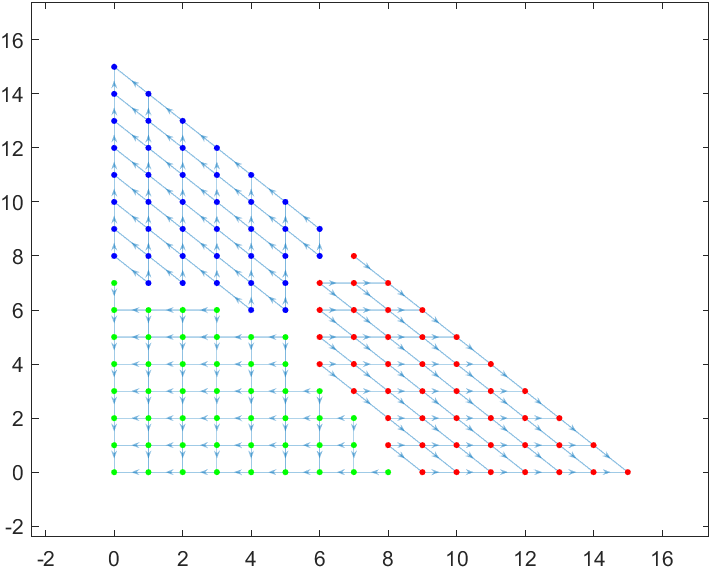
\includegraphics[width=0.7\linewidth]{TourTheImi_Ex1}
	\caption{\texttt{TourTheImi} Ex. 1\\ \texttt{ TourTheImi\_Ex1.m}}
	\label{fig:tourtheimiex1}
\end{figure}

	% TODO: \usepackage{graphicx} required

Βλέπουμε ότι ο γράφος χωρίζεται σε ξεχωριστά groups ανάλογα με την σύγκλιση τους . Φαίνεται πως υπάρχει μια 1 προς 1 σχέση μεταξύ της αρχικής και τελικής κατάστασης(μπορούμε να γνωρίζουμε σίγουρα που θα καταλήξει μια κατάσταση από την αρχική κατάσταση και μόνο)
\\
Έπειτα κάνουμε ένα πείραμα με 5 \texttt{TfT}, 5 \texttt{Per\_CD}, 5 \texttt{Gradual}
% TODO: \usepackage{graphicx} required
\begin{figure}[th!]
	\centering
	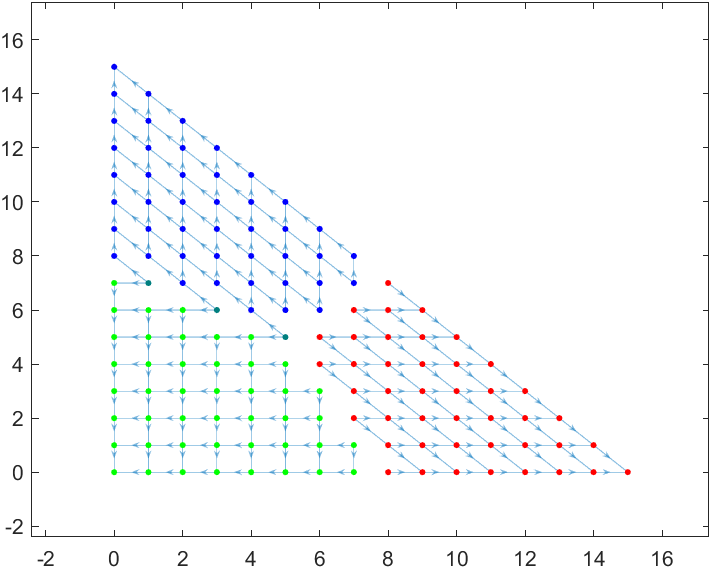
\includegraphics[width=0.7\linewidth]{TourTheImi_Ex2}
	\caption{\texttt{TourTheImi } Ex. 2    \texttt{TourTheImi\_Ex2.m}}
	\label{fig:tourtheimiex2}
\end{figure}

Εδώ βλέπουμε ότι, παρόλο που ο γράφος πάλι χωρίζεται σε groups, υπάρχει μια επικοινωνία μεταξύ των 2 από τα 3 groups . Συγκεκριμένα , οι καταστάσεις \([7,1,7]\) ,\([6,3,6]\) και \([5,5,5]\) έχουν πιθανότητα να οδηγηθεί τόσο στην κατάσταση \([15,0,0]\) όσο και στην κατάσταση \([0,0,15]\). Αυτό λογικά συμβαίνει καθώς οι στρατηγικές \texttt{Tit\_for\_Tat} και \texttt{Gradual} έχουν ίδιο συνολικό score και στις 3 αυτές καταστάσεις.\\
\\

Το επόμενο πείραμα αποτελείται από 3 \texttt{Soft\_major}, 2 \texttt{Per\_Nasty}, 1 \texttt{Per\_kind}.
% TODO: \usepackage{graphicx} required
\begin{figure}[th!]
	\centering
	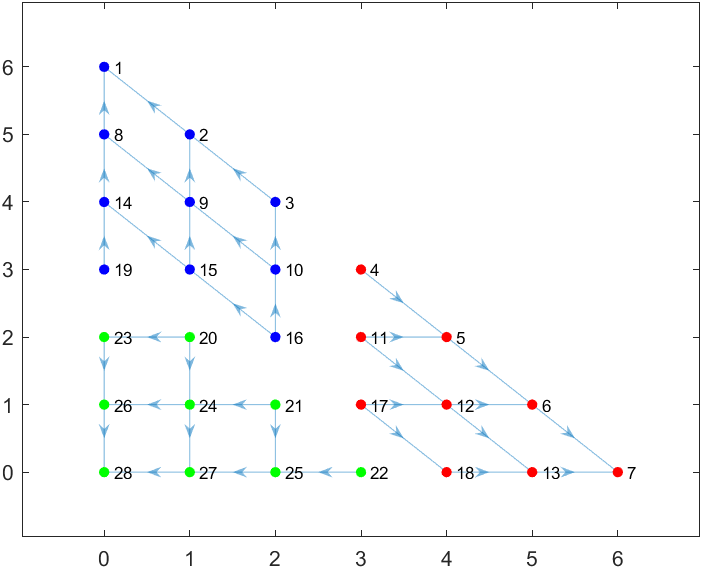
\includegraphics[width=0.6\linewidth]{TourTheImi_Ex3}
	\caption{\texttt{TourTheImi } Ex. 3 \texttt{ TourTheImi\_Ex3.m }}
	\label{fig:tourtheimiex3}
\end{figure}



Για την συνάρτηση \texttt{TourTheimi} δημιουργήσαμε μια δεύτερη παραλλαγή \nameref{appendix:TTI2} με τον εξής συλλογισμό: Το Score ενος πληθυσμού δεν θα έπρεπε να κρίνεται από τον αριθμό που τον εκπροσωπεί αλλά από την απόδοση ενός παίκτη.



Η μεγάλη διαφορά της \texttt{TourTheimi2} είναι ότι χρησιμοποιεί μια νέα συνάρτηση ( \nameref{appendix:Axel2Imp2}) για τον υπολογισμό του Score ανα στρατηγική , η οποία λαμβάνει υπόψη το Score μόνο ενός παίκτη.
\\
\\
Παμε να εξετάσουμε τα ίδια παραδείγματα με πάνω με την νέα συνάρτηση.
\\
\\
Δοκιμάζουμε με 5 \texttt{per\_CD},5 \texttt{soft\_major}, 5 \texttt{per\_nasty}.\\
\\
% TODO: \usepackage{graphicx} required
\begin{figure}[th!]
	\centering
	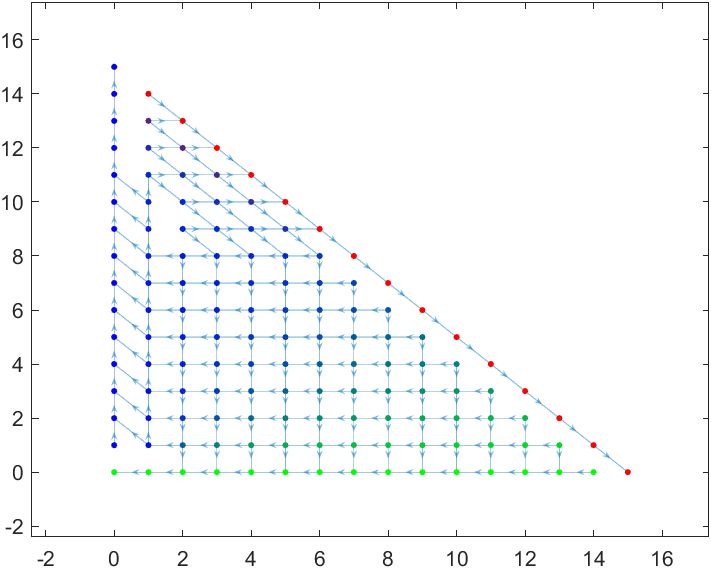
\includegraphics[width=0.7\linewidth]{TourTheImi_Ex1_2}
	\caption{\texttt{TourTheImi} Ex1\_2 \texttt{TourTheImi\_Ex1\_2.m}}
	\label{fig:tourtheimiex12}
\end{figure}
\\
Παρατηρούμε οτι το \texttt{TourTheImi2} έχει μεγάλη διαφοροποίηση. Εδω βλέπουμε ότι ο γράφος δεν χωρίζεται τόσο αισθητά σε Groups. Αυτό μας δείχνει πως υπάρχουν ισοδύναμες στρατηγικές στο συγκεκριμένο παράδειγμα.
\clearpage

Έπειτα έχουμε 5 \texttt{TfT}, 5 \texttt{Per\_CD}, 5 \texttt{Gradual}.
% TODO: \usepackage{graphicx} required
\begin{figure}[th!]
	\centering
	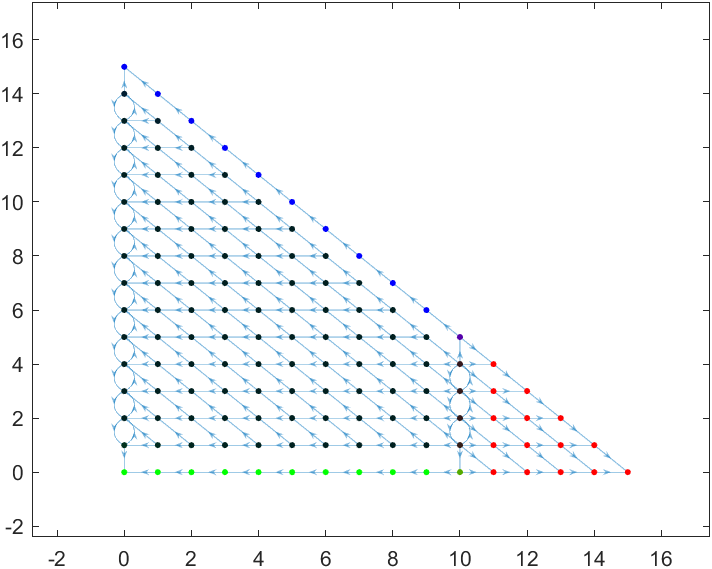
\includegraphics[width=0.7\linewidth]{TourTheImi_Ex2_2}
	\caption{\texttt{TourTheImi} Ex2\_2    \texttt{ TourTheImi\_Ex2\_2.m}}
	\label{fig:tourtheimiex22}
\end{figure}

Στο συγκεκριμένο παράδειγμα παρατηρούμε ότι στην περίπτωση που η στρατηγική \texttt{ Per\_CD} εκλείψει, οι στρατηγικές \texttt{Tit\_for\_Tat} και \texttt{Gradual} ταλαντεύονται στο ποιά θα υπερισχύσει. Επιπλέον στις καταστάσεις \([1,10,4]\),\([2,10,3]\),\([3,10,2]\) και \([4,10,1]\) βλέπουμε ότι από αυτές τις καταστάσεις μπορούμε να μετακινηθούμε προς πολλές κατευθύνσεις.\\
\\
Επόμενο πείραμα: 3 \texttt{Soft\_Major}, 2 \texttt{Per\_Nasty}, 1 \texttt{Per\_kind}

\begin{figure}[th!]
	\centering
	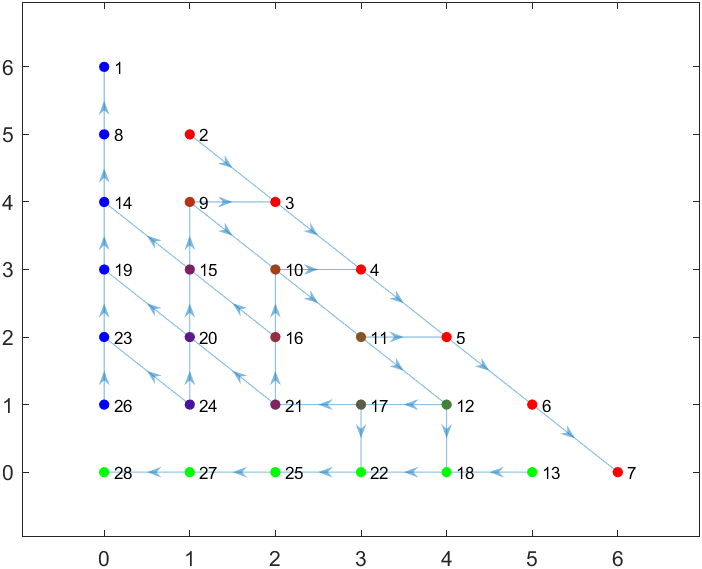
\includegraphics[width=0.60\linewidth]{TourTheImi_Ex3_2}
	\caption{\texttt{TourTheImi} Ex3\_2 \texttt{TourTheImi\_Ex3\_2.m}}
	\label{fig:tourtheimiex32}
	\flushleft
	Οπως και πριν , δεν παρατηρούμε κάτι ιδιαίτερο στο συγκεκριμένο πείραμα , ακόμα και με το TourTheImi2.
\end{figure}







\section{Προσομοίωση του Imitation Dynamics}
Ο κώδικας για το Simulation του Imitation Dynamics βρίσκεται εδω:\nameref{appendix:TourSimImi}
    
Η λογική είναι παρόμοια με την \nameref{appendix:TTI}, με την διαφορά ότι αυτή τη φορά δεν χρειάζεται να υπολογίσουμε τον πίνακα μεταβάσεων: Επιλέγουμε τυχαία \(Κ\) παίκτες και επιλέγουμε τυχαία μια από τις βέλτιστες στρατηγικές για να αλλάξουμε τους \( Κ\) παίκτες.
\\
\\
Εκτελώντας τα αντίστοιχα πειράματα με τη θεωρητική υλοποίηση παρατηρούμε ότι στην περίπτωση του Imitation όπου η βέλτιστη στρατηγική βρίσκεται από το συνολικό σκορ όλών των παικτών η συμπεριφορά του συστήματος εμφανίζει τις παρακάτω ιδιομορφίες:

\begin{enumerate}
\item  Στην περίπτωση που ένας πληθυσμός είναι αρχικά μεγαλύτερος από έναν άλλο, ο πληθυσμος τείνει να υπερισχύει έναντι των άλλων, όπως βλέπουμε στην 3η εικόνα που εκτελείται το χαοτικό πείραμα.

\item  Στην περίπτωση που οι πληθυσμοί είναι ίδιοι, τείνει να υπερισχύει αυτός που σε σχέση με το Theoretical Fitness εμφανίζει την πιο πρώιμη αύξηση. Αυτό μπορεί να οδηγήσει τόσο σε ορθή κατάταξη , όπως στην 2η εικονα στο πείραμα της μονότονης σύγκλισης, όσο και σε λανθασμένη , όπως στην πρώτη εικόνα με το πείραμα των ισχυρών αποστατών.


\end{enumerate}
Στην περίπτωση του Imitation όπου η βέλτιστη στρατηγική βρίσκεται από το σκορ του καλύτερου παίκτη, τα αποτελέσματα παρουσιάζονται πιο χαοτικά και δεν υπάρχει απαραίτητα μονοτονία στις μεταβολές όπως παρατηρείται στην πρώτη περίπτωση.\\
\\
% TODO: \usepackage{graphicx} required
\begin{figure}[!th]
	\centering
	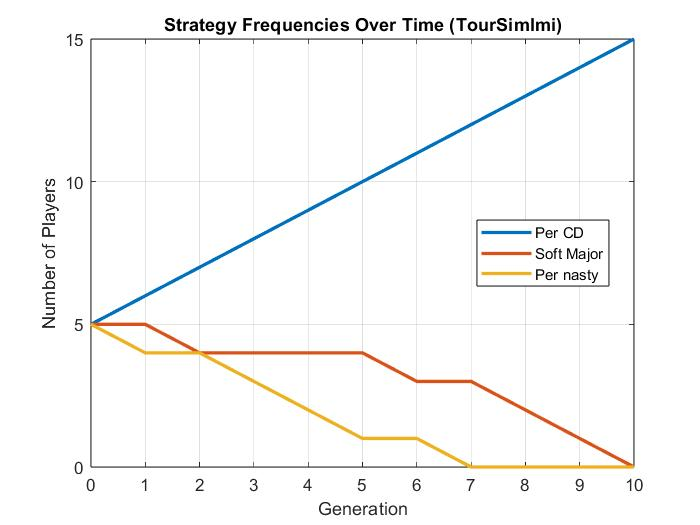
\includegraphics[width=0.7\linewidth]{toursimimi1}
	\caption{Convergence to the Final State \texttt{TourSimImi\_Ex1.m}}
	\label{fig:toursimimi1}
\end{figure}
% TODO: \usepackage{graphicx} required
\begin{figure}[ht!]
	\centering
	\begin{minipage}{0.48\textwidth}
		\centering
		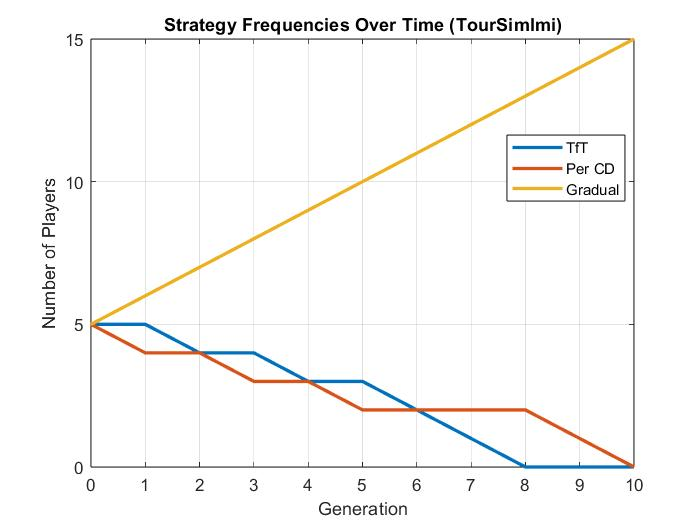
\includegraphics[width=0.8\linewidth]{toursimimi2}
	
	
	\end{minipage}
	\hfill
	\begin{minipage}{0.48\textwidth}
		\centering
		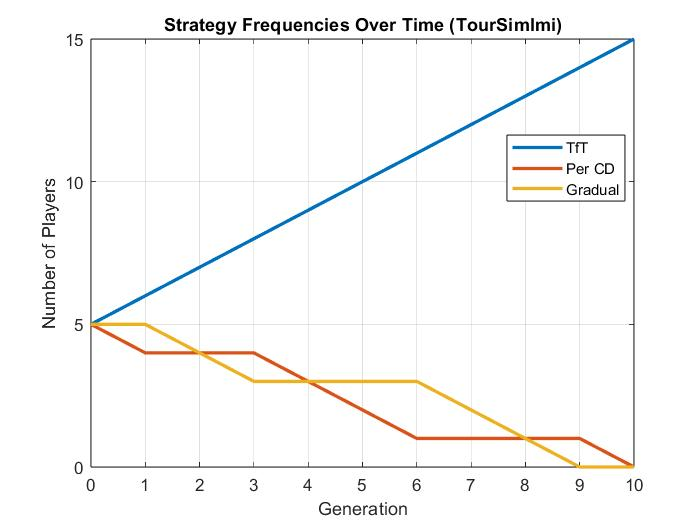
\includegraphics[width=0.8\linewidth]{toursimimi22}
	
	
	\end{minipage}
	\caption{Convergence of the states to the two possible final states shown by Markov Chain \texttt{  TourSimImi\_Ex2.m  }}
\end{figure}
% TODO: \usepackage{graphicx} required
\begin{figure}
	\centering
	
	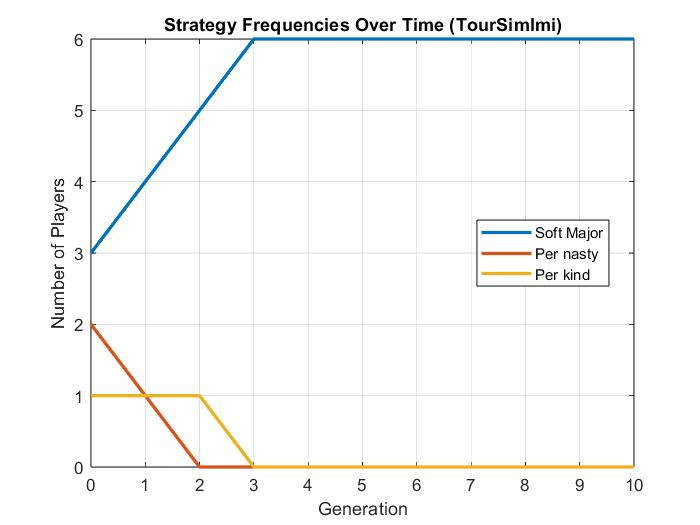
\includegraphics[width=0.7\linewidth]{toursimimi3}
	\caption{Convergence to the Final State   \texttt{(TourSimImi\_Ex3.m)}}
	\label{fig:toursimimi3}
\end{figure}
\clearpage
% TODO: \usepackage{graphicx} required
\begin{figure}
	\centering
	\begin{minipage}{0.48\textwidth}
		\centering
		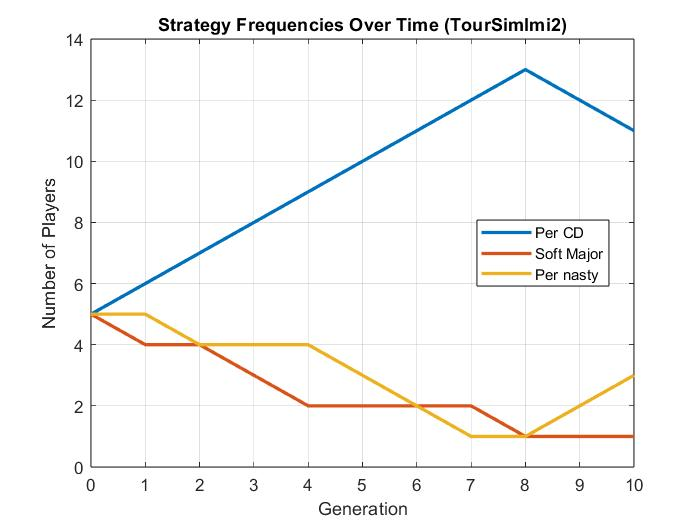
\includegraphics[width=0.7\linewidth]{toursimimi11.jpg}
	
		\label{fig:toursimimi11}
		
	\end{minipage}
		\begin{minipage}{0.48\textwidth}
			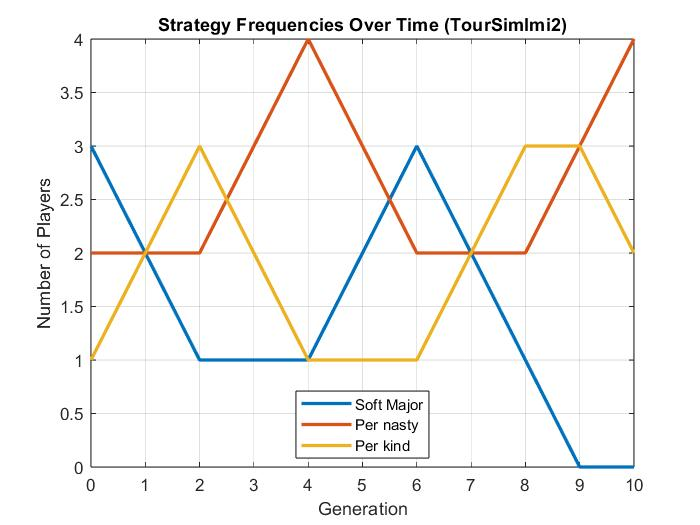
\includegraphics[width=0.7\linewidth]{toursimimi33}
			
		\end{minipage}
	
		\begin{minipage}{0.48\textwidth}
			\centering
		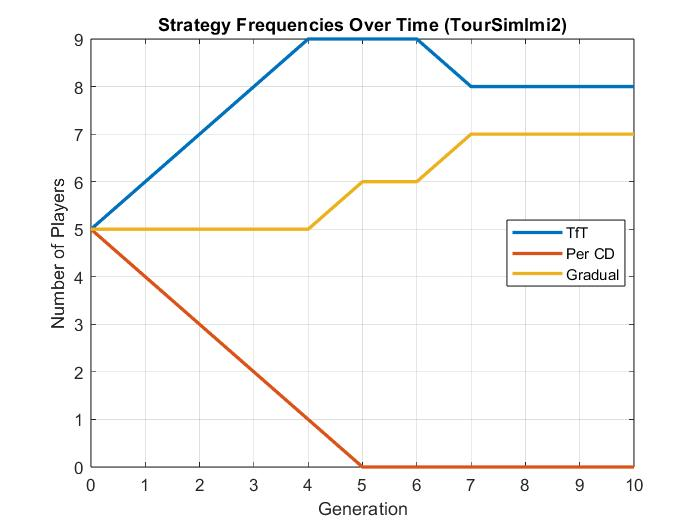
\includegraphics[width=0.7\linewidth]{toursimimi222}
	
	
	\end{minipage}
	\centering	
		\begin{minipage}{0.48\textwidth}
		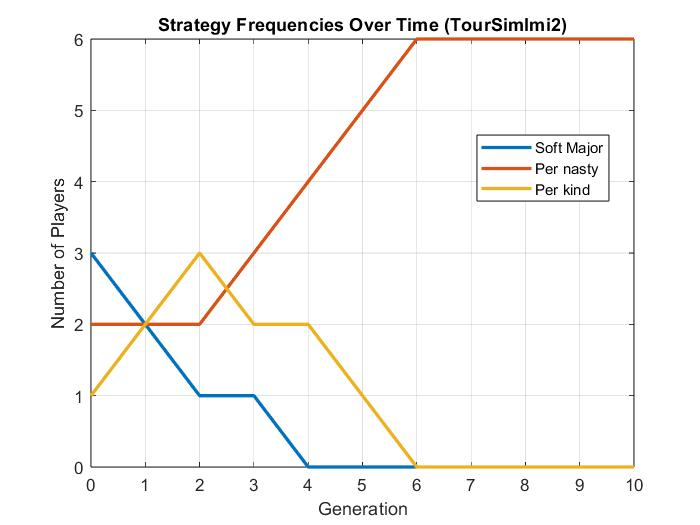
\includegraphics[width=0.7\linewidth]{toursimimi333}
		
	\end{minipage}
		\begin{minipage}{0.48\textwidth}
		\centering
		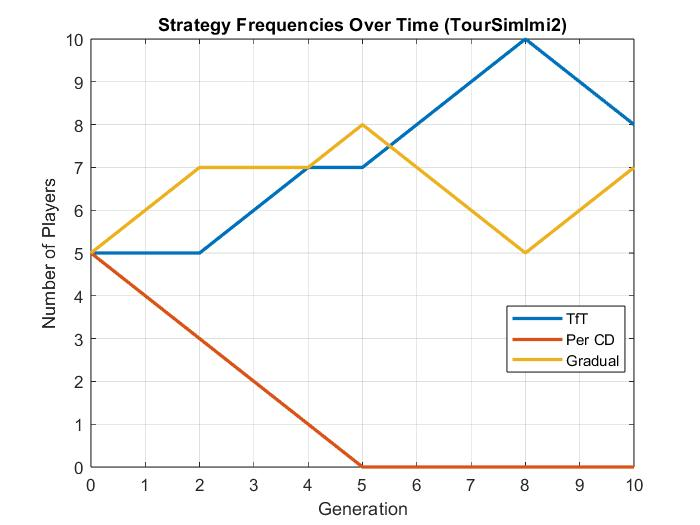
\includegraphics[width=0.7\linewidth]{toursimimi2222}
		
	\end{minipage}
	\caption{Increased Oscilations and random state transition using \texttt{TourSimImi2} \texttt{TourSimImi\_Ex1\_2.m, TourSimImi\_Ex2\_2.m,  TourSimImi\_Ex3\_2.m }}
\end{figure}
